\documentclass[12pt]{article}
\usepackage{graphicx}
\usepackage[section]{placeins}
\usepackage{amsmath}
\usepackage{enumitem}
\usepackage{tcolorbox}
\usepackage{subfigure}
\usepackage{amssymb}
\usepackage{hyperref}

\title{Controlled Procedural Terrain Generation}
\author{Alfredo Russo}
\date{A.A. 2021-2022}

\begin{document}
    \maketitle
    \newpage
    \tableofcontents
    \newpage
    

    \section{Introduction}

    \section{Coastline Agent}

    \section{Smoothing Agent}
    Smoothing agent is the one which deals with smoothing points previously elevated by the coastline agent.
    In order to do that it use extended Von Neumann neighborhood, changing the height of the points while it perform a random walk 
    on the map.
    
    \subsection{Agent parameter}
    Like every agent it has parameters that allow designer to lead different results based on it.
    These parameters are:
    \begin{itemize}
        \item \textbf{AgentNr:} it represents the number of agent that will be placed on the map in order to smooth coastline points.
        \item \textbf{returnValue:} this is a value used for understand when the agent have to came back to its starting point. The more the value is high, the more
        the points near the starting point will be smooth. So the agent came back to the starting point periodically and this is useful if some parts of the map need 
        more smoothing than others.
        \item \textbf{smoothingTokens:} it represents, like all other agent, the number of action that the agent can perform. The more the number is high, the more the map will be smooth.
    \end{itemize}

    For speeding up the computation there is another parameter taken by the coastline agent script which is \textbf{coastline points}, so the points where it is possible to place agents.
    This is done because retrieving coastline points (points which height is more than 0) can be performance expensive depending on how much the map is big. 

    \noindent 
    Smoothing agent require terrain to work, so there are all the parameters related to the terrain like \textbf{terrain data}, \textbf{heightmap} and so on \dots

    \noindent
    There is also a parameter called \textbf{neighboringPoint} which is used when the agent have to move itself in an adjacent point.
    
    \noindent
    At the end there is an instance of the smoothing agent in order to let the agent start working after and only after the coastline agent finish its work.

    \subsection{Action}
    This method represents the agent action on the map, but before it can start there are a couple of things to do.
    The first thing is to retrieve all the heights related to map points previously generated by the coastline agent. So the heightmap matrix is filled with this information.
    The second one is to retrieve all the coastline point (the point with heights greater than 0) in order to place the agents on the map. This is done by retrieving the
    related hashset by the coastline agent script in order to avoid useless computation. Furthermore, the complexity of this kind of computation increase with the map size 
    because it is needed to check every point height of the map.
    After these things the action can start.

    Every agent need to be placed on the map but not in a completely random way. The agents have to be placed on a coastline point, so in order to do that a random point is retrieved
    from the hashset which contains them and assigned to the starting point. This point is very important for the smoothing agent because, as previously said, this agent returns
    to its starting point periodically.

    In order to understand when the agent have to return to its starting point it is used a counter (\textbf{count}) originally set to 0;
    
    It is important to track the position of every agent and for this is used a variable called \textbf{location} that it is updated during time with the current agent position. 
    At the beginning it is set to the value of the starting point.

    Every agent can perform an action according to the number of the tokens specified. The action can consist of came back to the starting point or change the height of a point
    with extended VonNeumannNeighborhood.

    If the value specified as \textbf{returnValue} is 5, it means that the agent have to came back to the starting point 5 times. In order to compute after how many action the agent
    have to came back, the number of tokens is divided by the returnValue. So if the counter is greater than this value the agent have to came back, the location is set to the
    starting point and the counter is set to 0. Otherwise, the agent can perform its action computing the new height for the point where it is and then update the value in the heightmap.
    After this, the agent move itself on a valid random neighboring point thanks to the \textbf{GetNeighboringPoint} method and the counter is increased by one.

    I choose to use unity coroutine, so every time an agent end its work, the terrain is updated with the new heightmap values.

    \subsection{VonNeumannNeighborhood} \label{section:Von Neumann}
    The VonNeumannNeighborhood method compute the new height of the given point p as the average of points in an extended von Neumann neighborhood of p consisting of the
    four orthogonal map points surrounding p on the elevation grid and the four points beyond these, see figure \ref{fig:vonNeumann}.

    \begin{figure}
        \centering
        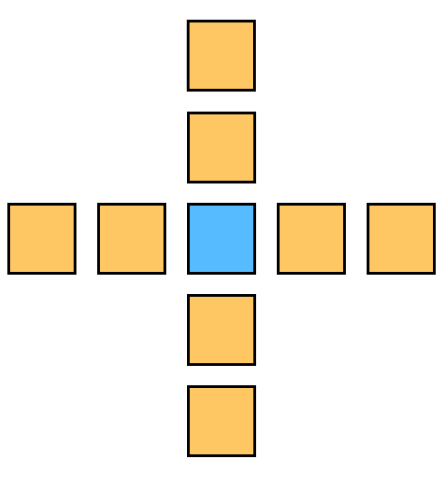
\includegraphics[scale = 0.7]{images/Extended VonNeumannNeighborhood.png}
        \caption{Extended Von Neumann Neighborhood}
        \label{fig:vonNeumann}
    \end{figure}

    \noindent
    A weighted average height is calculated, with the center point given 3 times the weight of the other points. Therefore, nine points with a total weight of eleven are used.
    Starting from this information it is possible to calculate the weight for the central point and the weight for the surrounding points resolving the following equation system:

    \begin{equation}
        \begin{cases}
            x + y = 11
            \\ 3x = y
        \end{cases}
    \end{equation}

    \noindent
    The variable x represents the weight for the central point which is 3 times the other points weight represented by y. So the central point weight is 11/4 and other points weight is 33/4.

    Then the heights of all the points are collected, but it can happen that a surrounding point of location is outside the map. In this case the height considered  is the location one. 
    This choice is done because otherwise the more the points are near to the end of the map, the more their heights will be near to zero, see figure \ref{fig:SmotthingCamparison}.
    
    \begin{figure}
        \centering     %%% not \center
        \subfigure[Height = 0]{\label{fig:Height0}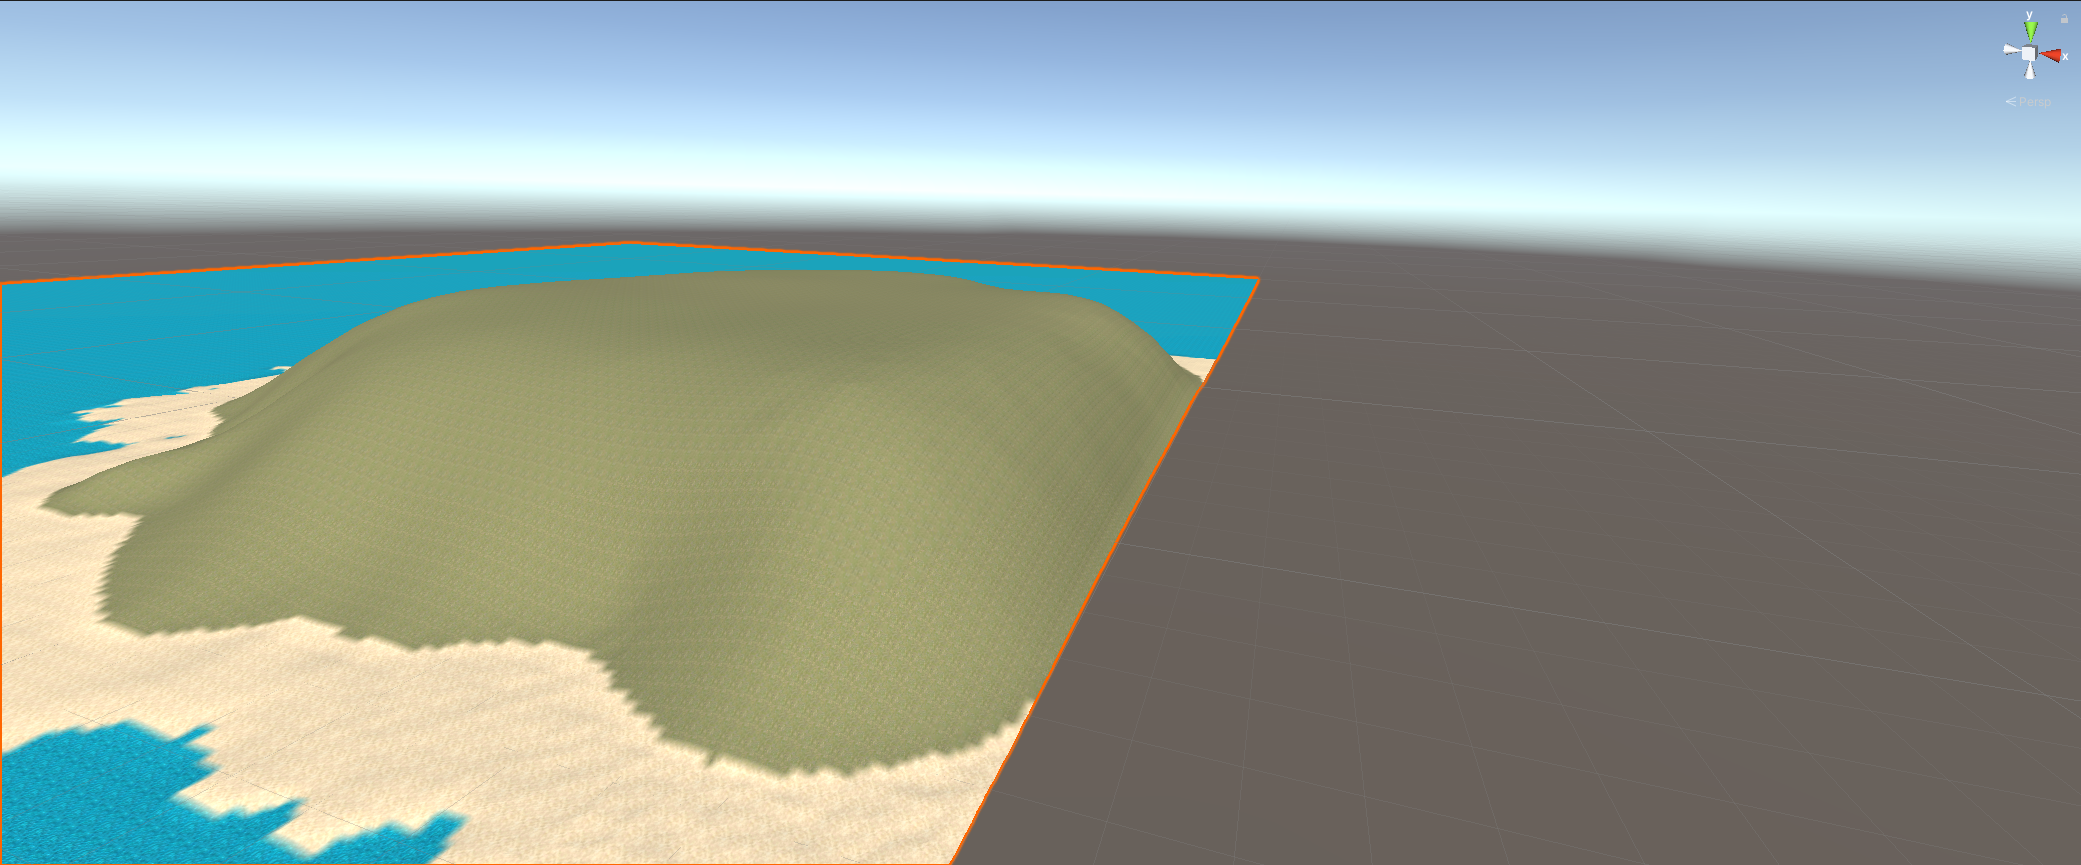
\includegraphics[width=60mm]{images/Smoothing agent height 0}}
        \subfigure[Height = location height]{\label{fig:LocationHeight}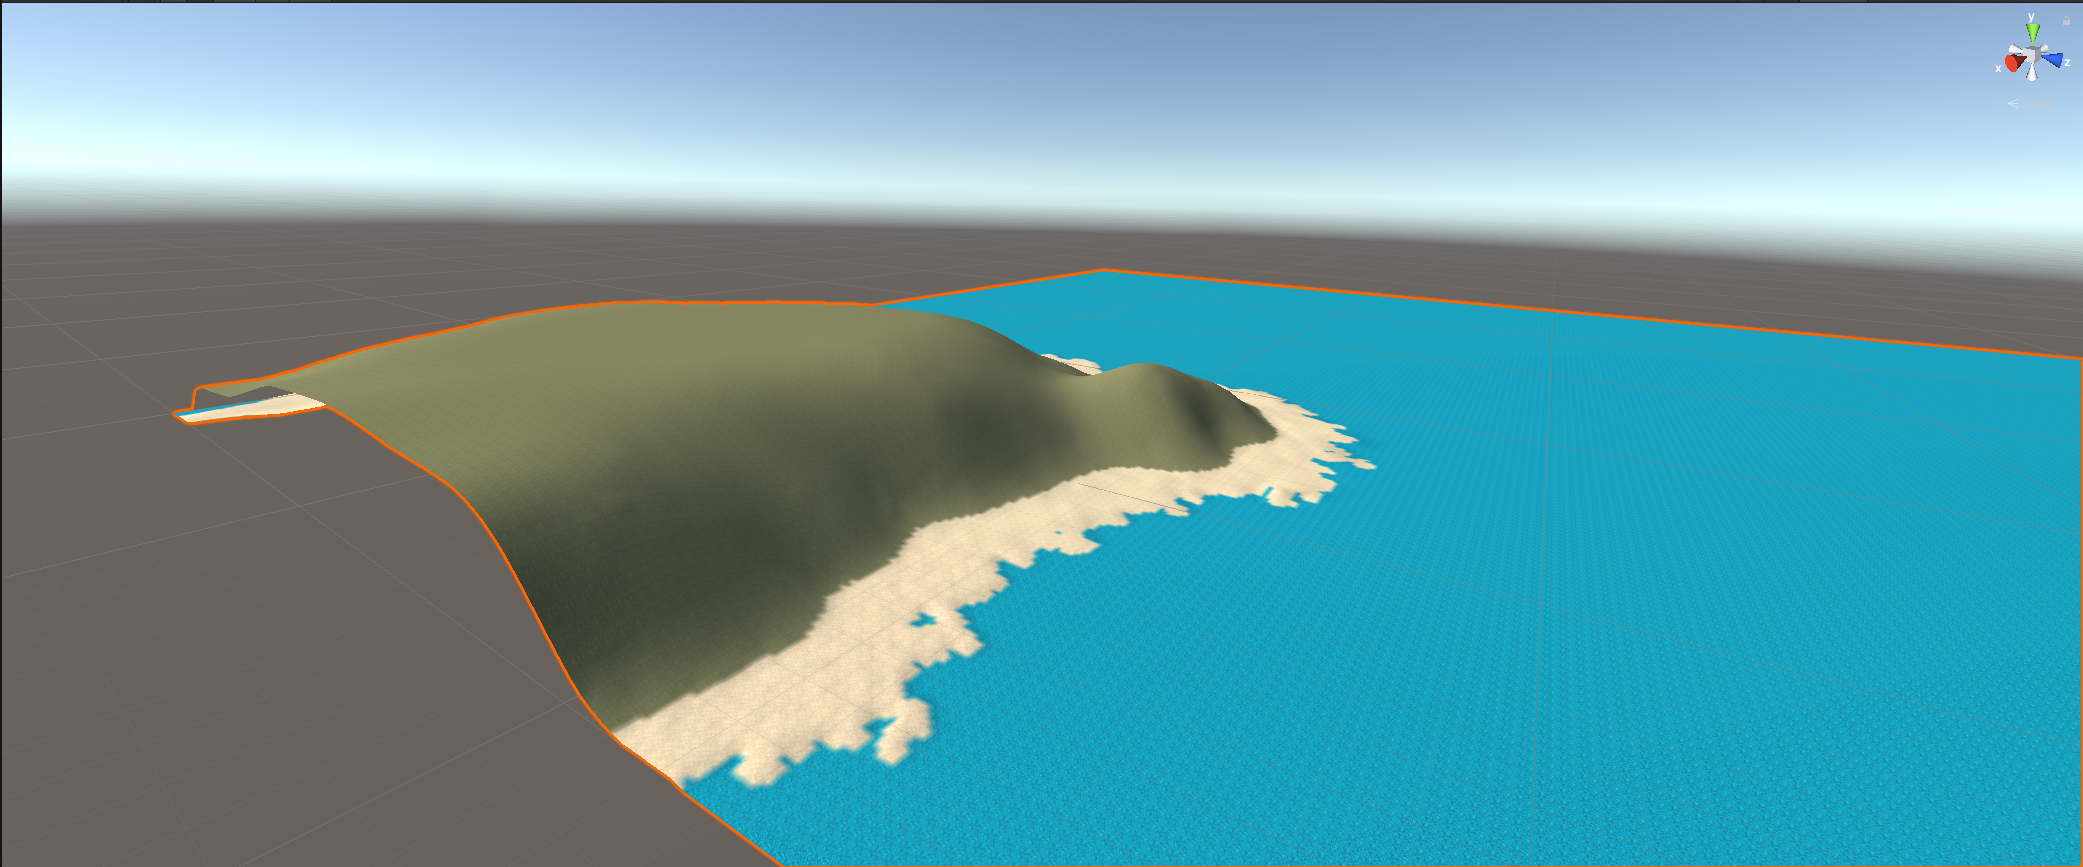
\includegraphics[width=60mm]{images/Smoothing agent height location}}
        \caption{Two different smoothing results.}
        \label{fig:SmotthingCamparison}
    \end{figure}
        
    
    After collected all heights the weighted average height is calculated as follows:

    \begin{equation}
        a = \dfrac{\sum\limits_{i=0}^{9} (W_i * H_i) }{ \sum\limits_{i=0}^{9} W_i }
    \end{equation}

    \noindent
    Where W represent the weight and H represent the height value related to the point. 

    \subsection{GetNeighboringPoint}
    This method takes the current location of the agent and starting from this check if the neighboring point are inside the terrain and then add it to a list. After it is chosen a 
    random point between the valid ones found.

    In order to check if a point is inside the terrain it is used the method called \textbf{IsInsideTerrain} that check if the coordinate of the point are between the range 0 and
    the limit of the map.

    \section{Beach Agent}
    This agent start its work after smoothing agent ends its own. In order to do that it is used an instance of the agent that allow to start the action after smoothing agent end its work.
    Beach agent has the work to generate beach according to the parameter chosen by the designer.
    According to this it is possible to obtain a very huge beach all around the coastline or small one in some part of it. It is also possible
    to have flat beach or one that allow fluctuation in its height.

    \subsection{Agent Parameter}
    The beach agent have the following parameter that designer can exploit to generate a different kind of beach:

    \begin{itemize}
        \item \textbf{beachAgentNr:} it represents the number of agent that will work for generating beach.
        \item \textbf{beachTokens:} it is the number of action that each agent have.
        \item \textbf{heightLimit:} it is the altitude limit, when the agent reaches a point higher than the limit specified, it leaves the area
        and move to another random shoreline point.
        \item \textbf{randomWalkSize:} when the agent is placed on a random shoreline point it jumps away from it changing the height of
        the point and smoothing them according to the parameters specified. How long will be its walk is specified by randomWalkSize parameter.
        \item \textbf{awayLimit:} when the agent have to jump away from the coastline it is needed to know how much far the agent have to jump away.
        So the awayLimit parameter it is really important since it specify that information.
        \item \textbf{beachHeight:} it is a range between [0.003, 0.01[ that represent beach height. Actually, in Unity, we are working with heightmap
        matrix where the heights are mapped inside the range 0-1. So the value previously written have to be multiplied by the maximum height of the 
        unity terrain. If the maximum height of the unity terrain is 100, the range previously specified becomes [0.3, 1[.
    \end{itemize}

    \subsection{Action}
    Before starting beach agent action, the heightmap matrix have to be filled with the value related to the points' height of unity terrain.
    
    \noindent
    After the smoothing agent action, it can happen that there are points with height between 0 and 0.003 which are neither sea point nor beach point. In 
    order to avoid this behavior a method called \textbf{FlatPoints} is invoked. This method set the height of those points to 0.
    In order to place the agent on the map and replace it when the agent get stuck, a list with all the shoreline points is used and filled thanks to \textbf{GetShorelinePoints}
    method.
    
    Every agent have to be placed on the map, so at the beginning it is retrieved a random shoreline point from the list previously mentioned, and the value is assigned to location
    which represents the current position of the agent that will change over time.

    After the agent is placed on the map it can start its work. The first things to do is to check if the location has an height value greater than the \textbf{heightLimit}.
    If it is, the agent have to be replaced on the map and its location is changed to another random shoreline point.
    
    Then location point and the surrounding points are flattened and this means that a random height value between the \textbf{beachHeight} range is assigned
    to them. After these points are smoothed using Von Neumann Neighborhood, see section \ref{section:Von Neumann}.

    Then the agent move itself to a random point away from the coast using \textbf{AwayRandomPoint} method. The new point is stored inside a different variable
    than location since after the agent ends its random walk, it has to came back to the location and move itself to another shoreline point near location.

    Now the agent is ready to start its random walk which duration depends on the parameter \textbf{randomWalkSize}. The agent start to flatten and smooth the away point
    and its neighboring point and only after it moves itself to a valid neighboring point exploiting \textbf{GetNeighboringPoint} method. A point is a valid one if it is 
    inside the map and its height is less than 0.01. It is possible that no valid point near the current position of the agent is found, if it happens means that the 
    agent isn't able to move itself to another point, so its random walk ends. For checking this, it is used a placeholder parameter which is the value Vector2Int.one.

    When the agent random walk ends the agent move itself to a new shoreline point near the shoreline point where it was before, assigning the new value to the 
    location variable.

    \subsection{CheckShorelinePoint}
    This method is used by \textbf{GetShorelinePoints} one in order to check if a point is a shoreline one or not. It returns true if the point has an height value
    between the range [0.003, 0.01[. This range was chosen so the points retrieved are point quite close to the sea. Another thing to check by this method is
    if the coordinate of the point plus the away limit are inside the map or not, in order to understand if the agent starting from this point is able to jump away from it.

    \subsection{GetNeighboringPoint}
    This method is used in order to retrieve a position where the agent can move itself exploiting \textbf{GetNeighboringPoints} method which return all
    valid points. If there are no valid points around the location a placeholder value is returned in order to communicate that the agent isn't able
    to move itself.

    \subsection{AwayRandomPoint}
    As previously said, this method allow the agent to jump away from the coast. It add to location a direction multiplied by the \textbf{awayLimit} in order
    to retrieve a point away from the coast and check if it is inside the terrain and its height is less than 0.01. It will be for sure a point away starting
    from the one given in input because every shoreline point can be called like this only if it allows jumping away from it. This check is done by 
    \textbf{GetShorelinePoints} method.

    \section{City Agent}
    City agent is responsible to create road and house on the coastline previously created by other agents. This agent can work only if the landmass generated
    is quite flat. 

    \subsection{Agent Parameter}
    \begin{itemize}
        \item \textbf{cityAgentNr:} it is the number of agent which will create the city. Every agent is responsible to create a city zone, the more this 
        number is high, the more the number of city zone will be. Depending on how much the landmass generated is big and how many points where to place road
        and house there are, an agent can add details to a zone previously generated by other agents.
        \item \textbf{cityTokens:} it is the number of action performable by the agent. An action for the agent is moving itself to a valid point and place road 
        and houses according to the following parameter.
        \item \textbf{roadGameObject:} it is the game object that represent the road. It is a simple unity quad.
        \item \textbf{houseGameObject:} the game object that represents house. It is used a simple unity cube with a red material attached on it, there is also a box collider
        in order to perform some checks which will be presented later.
        \item \textbf{gap:} this parameter represents the distance between one house and others. If the gap is equal to 1 the house will be placed side by side
        along the road. Insted if the gap is too high, it can be possible that there is not enough space in order to place houses. After the agent placed a road,
        at least one house is place at the middle of the road, see section \ref{section:CreateHouse}. 
        \item \textbf{roadLength:} it is a range between [5, 20] which specify how long the roads should be. If the length is too high related to the size of the landmass,
        the agent may fail to create a city since there isn't enough space. 
        \item \textbf{numberOfHouse:} This parameter is a dynamic one since it depends on the \textbf{roadLength} and \textbf{gap} specified earlier. In order to achieve this result in unity,
        the editor is changed, and int slider object is used. It requires a variable where the value will be stored, the left value for the slider which is 1, that
        represents the minimum number of house placeable and the right value which represents the maximum number of houses placeable. Actually, the right value parameter depends on
        the road lenght and gap parameters previously mentioned. So in the code there is a dynamic getter for the value \textbf{MaxHouse} which is like following:
        \begin{equation}
            MaxNHouse = \begin{cases} (roadLenght/gap) - 2, & \mbox{if } gap\mbox{ = 1} \\ (roadLenght/gap) - 1, & \mbox{} otherwise\  \end{cases}
        \end{equation}

        The gap equal to 1 means that the house can be placed side by side along the roads. The roads can be orthogonal between them, so the house, which position is 
        at the end of the roads, can be duplicated if the value returned is (roadLength/gap) - 1, see figure \ref{fig:cornerHouse}.
        
        \begin{figure}
            \centering
            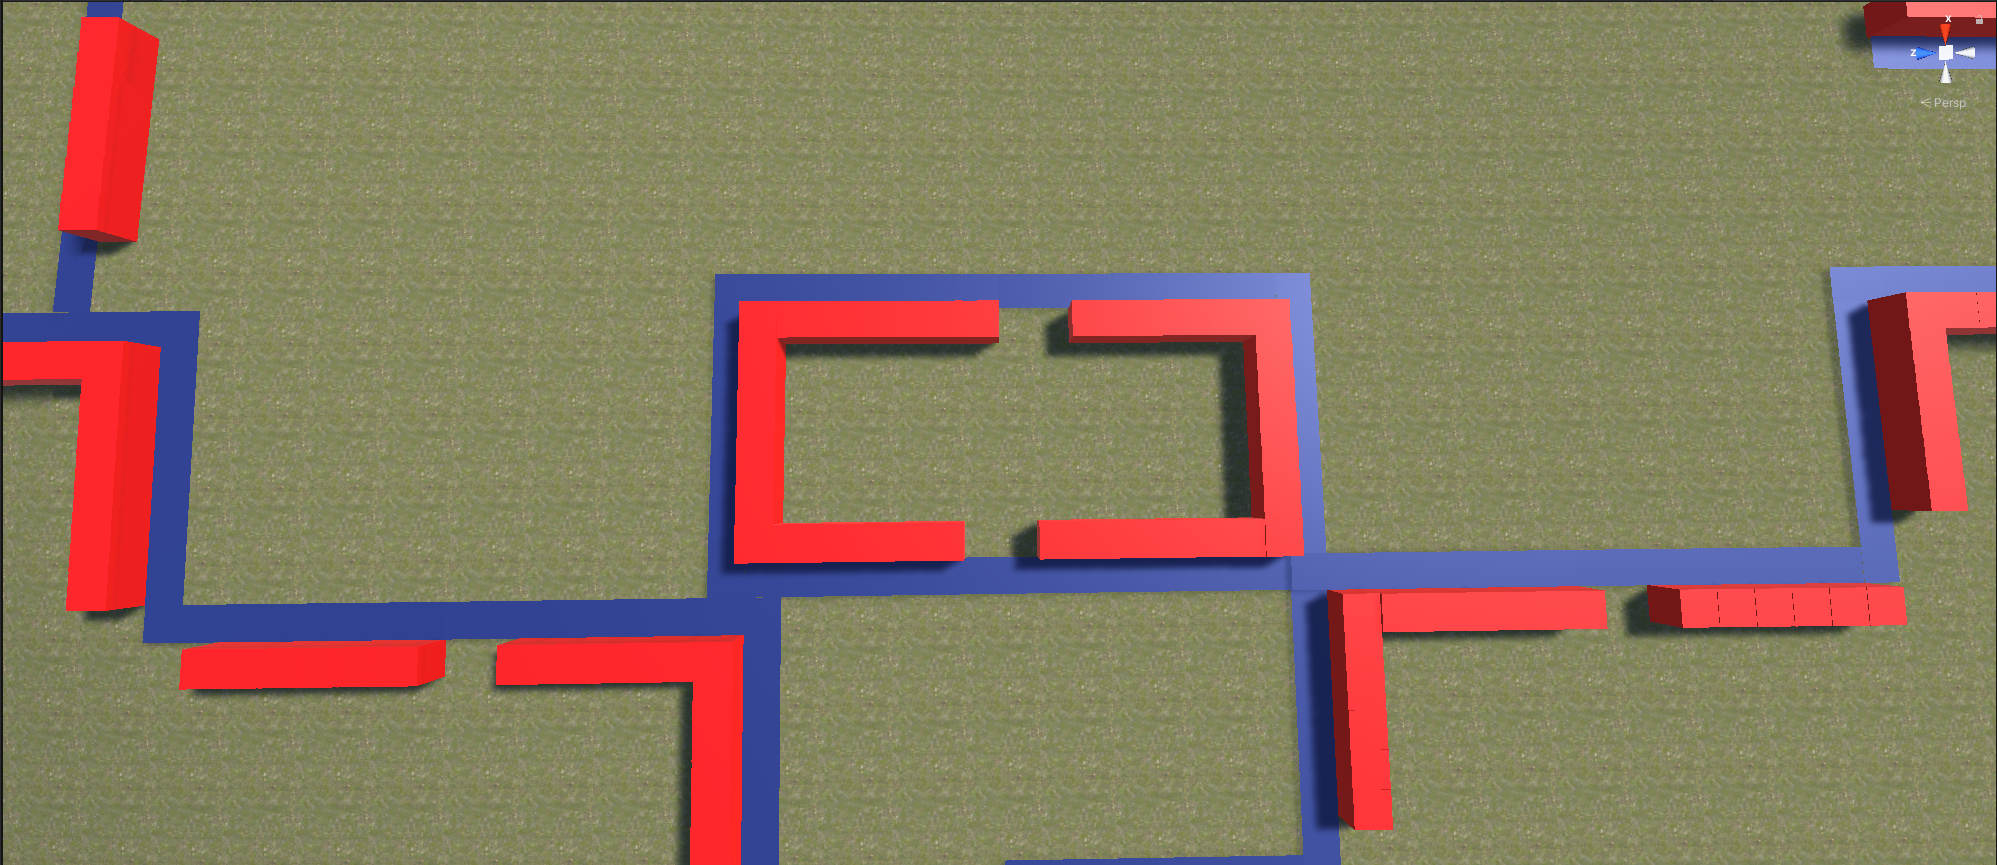
\includegraphics[scale = 0.19]{images/Corner house.png}
            \caption{Corner house}
            \label{fig:cornerHouse}
        \end{figure}
        
    \end{itemize}

    There is an instance of the city agent class since it start working only after the landmass is created, so after beach agent action.

    \subsection{Action} \label{seciton:action}
    As always before the city agent can start, it is needed that all the information about the height are putted inside the heightmap matrix after used
    for different check. There is another important thing to do before the agent can start, it is to retrieve all valid points where the agent can be placed on the
    map, so all valid where the agent can place road and house, see section \ref{section: ValidPoints}.

    Since unity terrain can be place at every position in the world, it is important to retrieve its position in order to place roads and house at right position on 
    terrain.

    Then every agent have to be placed on the map, in order to do that a random point from the list of all valid points is retrieved and assigned to location variable
    which represent the current position of the agent. In order to not let the agent come back to the previous location when it tries to move itself on the map, that
    position is keep inside \textbf{prevLocation} variable. At beginning this variable is set equal to location, in this way it is possible to understand if the agent
    has just been placed on the map, see section \ref{section:NewLocation}.

    Every agent has a number of tokens to consume which represents the action that can perform. An action for city agent is to place a road and the related number of
    house and then move itself to a valid point. In order to place the road two points are needed, from which a direction is extrapolated. This is done with the methods
    \textbf{CreateRoads} and \textbf{CreateHouse}, see \ref{section:CreateRoad} and \ref{section:CreateHouse}. Since it is used a unity coroutine the agent wait for a frame, and then 
    it moves itself to a new location thanks to \textbf{GetNewLocation} method, see \ref{section:NewLocation}. Before this, the current location of the agent
    is stored inside a temporary variable which value will be the one of the previous location, since the method \textbf{GetNewLocation} need it without being changed.
    If a new location is found the agent move itself to it and the previous location is updated with the value previously stored inside the temporary variable. Otherwise,
    no valid point is found, so the agent can't move itself to another point and its work ends. In order to check if the agent can move to another point or not, the 
    method \textbf{GetNewLocation} return the location given input, so the value returned is like the following:

    \begin{equation}
        location = \begin{cases} location, & \mbox{if } temporaryVariable { = location} \\ newLocation, & \mbox{} otherwise\  \end{cases}
    \end{equation}

    \subsection{Get Valid Points} \label{section: ValidPoints}
    In order to create a city there are some requirements to satisfy. The landmass have to be quite flat and the points considered must not be too steep.
    The first things to do is to considered all the landmass point and distinguish them from the other points like beach and sea one. To perform this task the
    average height of the points which height is greater than 0.01 is considered. So a landmass point is a point which height is greater than the average height plus
    0.05. This value was chosen after some test, it allows to not consider points that are too close to the beach. 

    Then is the time to check if the point consider is too steep or not. In order to do that the method \textbf{CheckStepness} is used. This method, thanks to a
    raycast which is located at position given in input but with a different height, check the angle between the normal of the point and the up vector. If the 
    angle is grater than 7, it means that the point is too steep for considering it as a good point to place road and house.
    
    So every map point is checked, and it can be considered a valid one only if its height is greater than the average one plus 0.05 and the angle between the normal 
    and the up vector is less than 7. A list with all valid points is returned.

    \subsection{Get New Location} \label{section:NewLocation}
    This method takes in input the current location of the agent and the previous one. It can happen that the value previously mentioned are the same. This is done in order
    to understand if the agent already started its work, or it has just been placed on the map. So if the agent already started its work, for retrieving position where it
    can move itself the method \textbf{GetCandidates} is used, the one which takes in input the current location of the agent and the previous one. Otherwise, the method
    \textbf{GetCandidates} which takes in input only the location is used. This is done because if the agent has just been placed on the map there are 4 points 
    where it can move itself, otherwise it can move itself only towards 3 points.
    
    Then those points have to be checked, this is done with \textbf{CheckCandidate} method, see \ref{section:CheckCandidate}. At the end it is returned a random point
    between the valid one found or the location given in input if there is neither one valid point where the agent can move itself.
     
    \subsection{Check Candidate} \label{section:CheckCandidate}
    It is used for check if the point considered is a valid one or not. This method takes two input, location which represents where the agent can move itself and 
    previous location which represents the current location of the agent.

    The first thing to do is to check if the location is inside terrain, but this time, unless the others, as upper bound it is used the size of the map minus 1. This is done
    because the point retrieved is a point where the road will be placed, since the houses are placed to the edge of the road considering the border like previously said
    lead to avoid placing houses outside the map. For the same reason the lower bound start from 1 instead of 0, so any point which has 0 inside coordinate isn't a valid one.

    Then it is needed to check the location steepness, this is done thanks to \textbf{CheckSteepness} method previously mentioned, see \ref{seciton:action}.

    Since a road can be placed only given two points, and it will be placed along all the point between them, it is needed to check if on the point along the direction
    from the previous location (current position of the agent) and location (the possible future position of the agent) there is something that will make location not 
    a valid point. For every point between location and previous location, it is checked to its right and left and twice its right and left, if there is another point where
    a road is placed. This is done because the house are placed at the edge of the road, so in order to avoid house collision every road need an empty space along
    its edge. So if there is a point to its right or left \textbf{or} twice its right or left, the location considered is not a valid one. Instead, if there is a road to
    its right and left \textbf{and} twice its right and left means that there is a road which will intersect the future one between previous location and location with a 
    90-degree angle, and this is a wanted behavior. When the agent check for a candidate point, the one to its right and left are always with a 90-degree angle. 
    In order to avoid checking left and right points near previous location, since there is almost surely a road to its right or left, checking points start from the 
    following point towards direction.
    
    At the end it is checked if along the point between location and previous location there is already another road.

    \subsection{Create Road} \label{section:CreateRoad}
    This method, starting from the location where the agent is, the previous location and terrain position place a road on terrain. The first thing done is to retrieve 
    world coordinate (Vector3) of location and previous location from terrain one (Vector2). Then a direction, from previous location to location, is computed as well as the distance
    between them. Before it is possible to instantiate the road it is needed to compute its rotation and scaling. For the rotation it is used the 
    method called \textbf{Quaternion.LookRotation} which take in input the direction in which the road have to look at and the up vector. Then it is computed the Vector3
    related to scaling which the first two coordinates are settled to 1 and the Z one is settled to the length of the road. At this point the road is instantiated on the previous
    location with rotation and scaling previously computed. Then it is translated to middle point between previous and current location and a bit up in order to not have the 
    road colliding with terrain.

    \subsection{Create House} \label{section:CreateHouse}
    It receives in input, as the previous method, the previous and current location and terrain position. Then the world coordinates of previous and current location are 
    computed like the direction from previous to current location. The first house is placed all the times to the middle of the road, so this point is found using the \textbf{Lerp}
    function between previous and current location. Then the rotation is calculated, as previously for the road, with \textbf{Quaternion.LookRotation} method, this time as the
    first input is given the cross product between the direction vector and the up vector. Since the cross product give back the orthogonal vector between the two in input
    it is retrieved perpendicular direction than the direction. So the house ``will always look'' the roads as well as the forward vector. Thanks to that, the house is
    translated to one unit behind using \textbf{-Vector3.forward}. If the parameter related to the number of house to place is equal to 1 means that the work of the agent ends, 
    otherwise the position for the other house have to be computed. 
    
    Other houses are place first to the right and then to the left of the first one placed, until the number of house which have to be placed is reached. The right direction in which
    the houses have to be places is the same as the direction computed from previous and current location, while left one is the inverse of it. So, starting from the first house position,
    the new position is calculated exploiting the directions previous mentioned according to the gap parameter. Since, as house, it is used a cube, all of them are translated 0.5 upward
    avoiding collision with terrain.

    \section{Tree Agent}
 
    \section{Harbor Agent}

\end{document}